\documentclass[a5paper,english,spanish,brazil]{ufsc-thesis}

	% ---
	% PACOTES
	% ---

	% ---
	% Pacotes fundamentais 
	% ---
	%\usepackage{lmodern}			% Usa a fonte Latin Modern			
	\usepackage[T1]{fontenc}		% Selecao de codigos de fonte.
	\usepackage[utf8]{inputenc}		% Codificacao do documento (conversão automática dos acentos)
	\usepackage{lastpage}			% Usado pela Ficha catalográfica
	\usepackage{indentfirst}		% Indenta o primeiro parágrafo de cada seção.
	\usepackage{color}				% Controle das cores

	\usepackage{graphicx}			% Inclusão de gráficos
	\usepackage{subfig}  % usar subfloat duas figuras na mesma figura
	\newcommand{\subfigureautorefname}{\figureautorefname} % fez funcionar o auto ref nas subfiguras

	%\renewcommand\theparagraph{\alph{paragraph})} %fazer o \paragraph virar enumerada por letra (a,b,c)

	\usepackage{microtype} 			% para melhorias de justificação
	\usepackage{mathtools} %para usar equations
	\usepackage{xfrac} %para usar \sfrac
	\everymath{\displaystyle} %força todas as expressões nem estilo de maior fonte
	%\usepackage{pslatex} % Coloca as letras em Times New Roman, mas não nos Títulos de seções e Capítulos 
	\usepackage{listings}
	\usepackage{listingsutf8}

	\usepackage{longtable}
	\usepackage{tabularx}

	\usepackage[framemethod=tikz]{mdframed} %destaque de prágrafos

	\graphicspath{{figuras/}}
	% ---
			
	% ---
	% Pacotes adicionais, usados apenas no âmbito do Modelo Canônico do abnteX2
	% ---
	\usepackage{lipsum}				% para geração de dummy text
	% ---

	% ---
	% Pacotes de citações
	% ---
	\usepackage[brazilian,hyperpageref]{backref}	 % Paginas com as citações na bibl
	\usepackage[alf]{abntex2cite}	% Citações padrão ABNT


	% ---
	% Informações de dados para CAPA e FOLHA DE ROSTO
	% ---
	\titulo{Repotencialização em Subestações de Alta Tensão Utilizando Módulos de Manobra Híbridos Compactos}
	\autor{Joan Francisco {}Alvarez Burgos}
	\local{Florianópolios, SC-Brasil}
	\data{\today}
	\orientador{Maurício Valencia {}Ferreira da Luz}
	%\coorientador{Equipe \abnTeX}
	%\instituicao{
	%  Universidade Federal de Santa Catarina -- UFSC
	%  \par
	%  Centro Tecnológico -- CTC
	%  \par
	%  Departamento de Engenharia Elétrica -- EEL}
	\instituicao{Universidade Federal de Santa Catarina}
	\centro{Centro Tecnológico -- CTC}
	\programa{Programa de Graduação em Engenharia Elétrica}
	\assuntos{Subestações,Sistemas de Potência,Instalações Elétricas,Orçamentos}
	\tipotrabalho{Trabalho de Conclusão de Curso}
	% O preambulo deve conter o tipo do trabalho, o objetivo, 
	% o nome da instituição e a área de concentração 
	\preambulo{Monografia submetida ao Programa de Graduação em Engenharia Elétrica da Universidade Federal de Santa Catarina como requisito para aprovação na disciplina EEL7890 -- Trabalho de Conclusão de Curso (TCC).}
	% ---


	% ---
	% Configurações de aparência do PDF final

	% alterando o aspecto da cor azul
	\definecolor{blue}{RGB}{6,69,173} %padrão wikipedia de cor de link

	% informações do PDF
	\makeatletter
	\hypersetup{
	     	%pagebackref=true,
			pdftitle={\@title}, 
			pdfauthor={\@author},
	    	pdfsubject={\imprimirpreambulo},
		    pdfcreator={LaTeX with abnTeX2},
			pdfkeywords={abnt}{latex}{abntex}{abntex2}{trabalho acadêmico}, 
			colorlinks=true,       		% false: boxed links; true: colored links
	    	linkcolor=blue,          	% color of internal links
	    	citecolor=blue,        		% color of links to bibliography
	    	filecolor=magenta,      		% color of file links
			urlcolor=blue,
			bookmarksdepth=4
	}
	\makeatother
	% --- 

	% ---
	% compila o indice
	% ---
	\makeindex
	% ---

	% ----
	% Início do documento
	% ----
	\begin{document}
	% Retira espaço extra obsoleto entre as frases.
	\frenchspacing 

	% ----------------------------------------------------------
	% ELEMENTOS PRÉ-TEXTUAIS
	% ----------------------------------------------------------
	\pretextual

	% ---
	% Capa
	% ---
	\imprimircapa
	% ---

	% ---
	% Folha de rosto
	% (o * indica que haverá a ficha bibliográfica)
	% ---
	\imprimirfolhaderosto*
	% ---

	%\clearpage
	\imprimirfichacatalografica

	% ---
	% Inserir folha de aprovação
	% ---

	% Isto é um exemplo de Folha de aprovação, elemento obrigatório da NBR
	% 14724/2011 (seção 4.2.1.3). Você pode utilizar este modelo até a aprovação
	% do trabalho. Após isso, substitua todo o conteúdo deste arquivo por uma
	% imagem da página assinada pela banca com o comando abaixo:
	%
	% \includepdf{folhadeaprovacao_final.pdf}
	%
	\begin{folhadeaprovacao}

	  \begin{center}
	    {\imprimirautor}

	    \vspace*{\fill}\vspace*{\fill}
	    \begin{center}
	      \ABNTEXchapterfont\bfseries\Large\imprimirtitulo
	    \end{center}
	    \vspace*{\fill}
	    
	    %\hspace{.45\textwidth}
	    
	    	\begin{center}
	    		\vspace*{0.5cm}
	    		Esta Monografia foi julgada no contexto da disciplina EEL7890 -- Trabalho de Conclusão de Curso (TCC), e aprovado em sua forma final pelo Programa de Engenharia Elétrica da Universidade Federal de Santa Catarina.
	    		\vspace*{0.5cm}
	  		\end{center}
	    
	    \vspace*{\fill}
	   \end{center}
	  
	  \begin{center}
	    %\vspace*{0.5cm}
	    {\large\imprimirlocal},
	    {\large\imprimirdata}
	    %\vspace*{1cm}
	  \end{center}
	        
	   \assinatura{\textbf{ Prof. Dr. Eng. Renato Lucas Pacheco} \\ Coordenador de Graduação}
	   Banca Examinadora:
	   \assinatura{\textbf{Prof. Dr. Eng. \imprimirorientador} \\ Orientador} 
	   \assinatura{\textbf{Professor} \\ Convidado 1}
	   \assinatura{\textbf{Professor} \\ Convidado 2}
	   %\assinatura{\textbf{Professor} \\ Convidado 3}
	   %\assinatura{\textbf{Professor} \\ Convidado 4}
	      

	\end{folhadeaprovacao}
	% ---

	% ---
	% Dedicatória
	% ---
	\begin{dedicatoria}
	   \vspace*{\fill}
	   \centering
	   \noindent
	   \textit{Este trabalho é dedicado à minha família que foram tão compreensíveis e me deram tanto apoio nos momentos difíceis da jornada da graduação} \vspace*{\fill}
	\end{dedicatoria}
	% ---

	% ---
	% Agradecimentos
	% ---
	\begin{agradecimentos}
	\begin{mdframed}[hidealllines=true,backgroundcolor=blue!20]
	\lipsum[1]
	\end{mdframed}
	\end{agradecimentos}
	% ---

	% ---
	% Epígrafe
	% ---
	\begin{epigrafe}
	    \vspace*{\fill}
			\noindent
			\hangindent=5cm \\
	  \textit{`` O homem disse que tinha de ir embora -- antes queria me ensinar uma coisa muito importante: -- Você quer conhecer o segredo de ser um menino feliz para o resto da sua vida? \\ -- Quero -- Respondi. \\ O segredo se resume em três palavras, que ele pronunciou com intensidade, mãos nos meus ombros e olhos nos meus olhos: \\ -- Pense nos outros.''}
	    \begin{flushright}
			Fernando Sabino	
			\end{flushright}		
	\end{epigrafe}
	% ---

	% ---
	% RESUMOS
	% ---

	% resumo em português
	%\setlength{\absparsep}{18pt} % ajusta o espaçamento dos parágrafos do resumo
	%\begin{resumo}
	%Aqui vai o resumo

	% \textbf{Palavras-chaves}: latex. abntex. editoração de texto.
	%\end{resumo}

	% resumo em inglês
	%\begin{resumo}[Abstract]
	% \begin{otherlanguage*}{english}
	%   This is the english abstract.

	%   \vspace{\onelineskip}
	 
	%   \noindent 
	%   \textbf{Key-words}: latex. abntex. text editoration.
	% \end{otherlanguage*}
	%\end{resumo}


	% ---
	% inserir lista de ilustrações
	% ---
	\pdfbookmark[0]{\listfigurename}{lof}
	\listoffigures
	\cleardoublepage
	% ---

	% ---
	% inserir lista de tabelas
	% ---
	\pdfbookmark[0]{\listtablename}{lot}
	\listoftables*
	\cleardoublepage
	% ---

	% ---
	% inserir lista de abreviaturas e siglas
	% ---
	\begin{siglas}
	  \item[Celesc] Centrais Elétricas de Santa Catarina
	  \item[SE] Subestação
	  \item[CBU] Camboriú
	  \item[CMB] Camboriú Morro do Boi
	\end{siglas}
	% ---

	% ---
	% inserir lista de símbolos
	% ---
	\begin{simbolos}
	  \item[$ \Omega $] Letra grega Ômega
	  \item[$ \Delta $] Letra grega Delta
	\end{simbolos}

	% ---
	% inserir o sumario
	% ---
	\pdfbookmark[0]{\contentsname}{toc}
	\tableofcontents*
	\cleardoublepage
	% ---
%fim dos elementros Pré Textuais


% ----------------------------------------------------------
% ELEMENTOS TEXTUAIS
% ----------------------------------------------------------
\textual %isto faz as páginas dos elementos textuais serem numeradas

% ----------------------------------------------------------
% Introdução
% ----------------------------------------------------------
\chapter[Introdução]{Introdução} %o asterisco exclui a numeração e retira do sumário
	%\addcontentsline{toc}{chapter}{Introdução} %este volta a adicionar ao sumário a introdução
	O estudo de caso consiste na ampliação da Subestação Camboriú de responsabilidade das Centrais Elétricas de Santa Catarina – Celesc que opera em plena carga de 30MVA segundo dados do Centro de Operação do Sistema Elétrico da Celesc desde final de 2013.

	\section{Motivação}
		O acadêmico teve a possibilidade de realizar o programa de estágio na empresa Celesc Distribuição S.A. na Divisão de Subestações que possibilitou o contato com projetos de todo o estado de Santa Catarina. \par
		Com o crescente aumento da demanda no município de Balneário Camboriú e os sucessivos cortes não intencionais de energia no verão de 2013/2014 visto que a população pode variar de 100 mil habitantes para expressivos 1 milhão nas festas de fim de ano.\par
		A nova tecnologia de Módulo de Manobra Híbridos Compactos que integram dentro de si todas as funções de manobra como: disjuntor, seccionadoras, chaves de aterramento, terminais de vedação de cabos, interruptores de chaveamento rápidos e TPs, exceto TCs do tipo anel e dito híbridos, pois combinam as tecnologias Air Insulated System (AIS) e Gas Insulated System (GIS) que utiliza gás SF6 trazendo assim o que tem de melhor das duas tecnologias com confiabilidade e robustez do sistema.\par
		Somando que esta tecnologia tem sido implantada em subestações compactas com tecnologia RDS na Subestação Bombinhas e em subestações abrigadas como a Subestação Agronômica.

	\section{Objetivos}
		O projeto visa estudar a implantação e execução do projeto já realizado pela Divisão de Planejamento e Normas, enumeração e função de componentes da subestação e principalmente estudar a solução que foi lançada com o objetivo de ampliar de 30MVA para 75MVA até final de 2015 e possibilidade de ampliação futura para até 100MVA utilizando o mesmo pátio de manobra, ou seja, utilizando o mesmo terreno que encontra sem espaço físico para abrigar mais equipamentos que não sejam compactos.

	\section{Metodologia}
	\lipsum[1]

	% ---------------------------------------------------
	% Capítulo 1
	% ---------------------------------------------------

% ---------------------------------------------------
% Capítulo 1
% ---------------------------------------------------

\chapter{Equipamentos de Subestações}
	\label{chap:equipSE}
	Inicialmente para melhor elucidar o trabalho proposto faz-se necessário uma descrição inicial do que é uma subestação e a enumeração dos seus principais equipamentos que a compõe. Somente no \autoref{chap:projSEAT} se fará uma descrição da maneira como esses equipamentos podem ser arranjados para melhor confiabilidade do sistema.
	\section*{Subestação}
	Uma Subestação é um conjunto de condutores, aparelhos e equipamentos destinados a modificar as características da energia elétrica de tensão e corrente, permitindo a sua distribuição aos pontos de consumo em níveis adequados de utilização.\cite{instElet}

	\section{Para-Raios}
		O para-raios (mostrado na \autoref{fig:pararaioA}) é um equipamento de proteção principalmente constituído por uma série de varistores\footnote{Um componente elétrico que varia sua resistência conforme a tensão aplicada\cite[p. 413]{BellSytemHistory}} de alta potência colocados em série, projetado para reduzir o nível dos surtos de sobretensão a valores compatíveis com a suportabilidade desses sistemas provenientes principalmente de descargas atmosféricas.\par
		Os para-raios utilizam a propriedade de não linearidade dos elementos que são fabricados para conduzir a corrente de descarga associados às tensões induzidas nas redes, em seguida interromper as correntes subsequentes e conduzi-las à terra.\par
		Estes são construídos por meio da escolha de dos materiais: o carbonato de silício (SiC) ou óxido de zinco (ZnO). 

		\begin{figure}[htb]
			\caption{Para-raios e sua placa de identificação}
			\centering
			\subfloat[Para-raio de Potência] {
			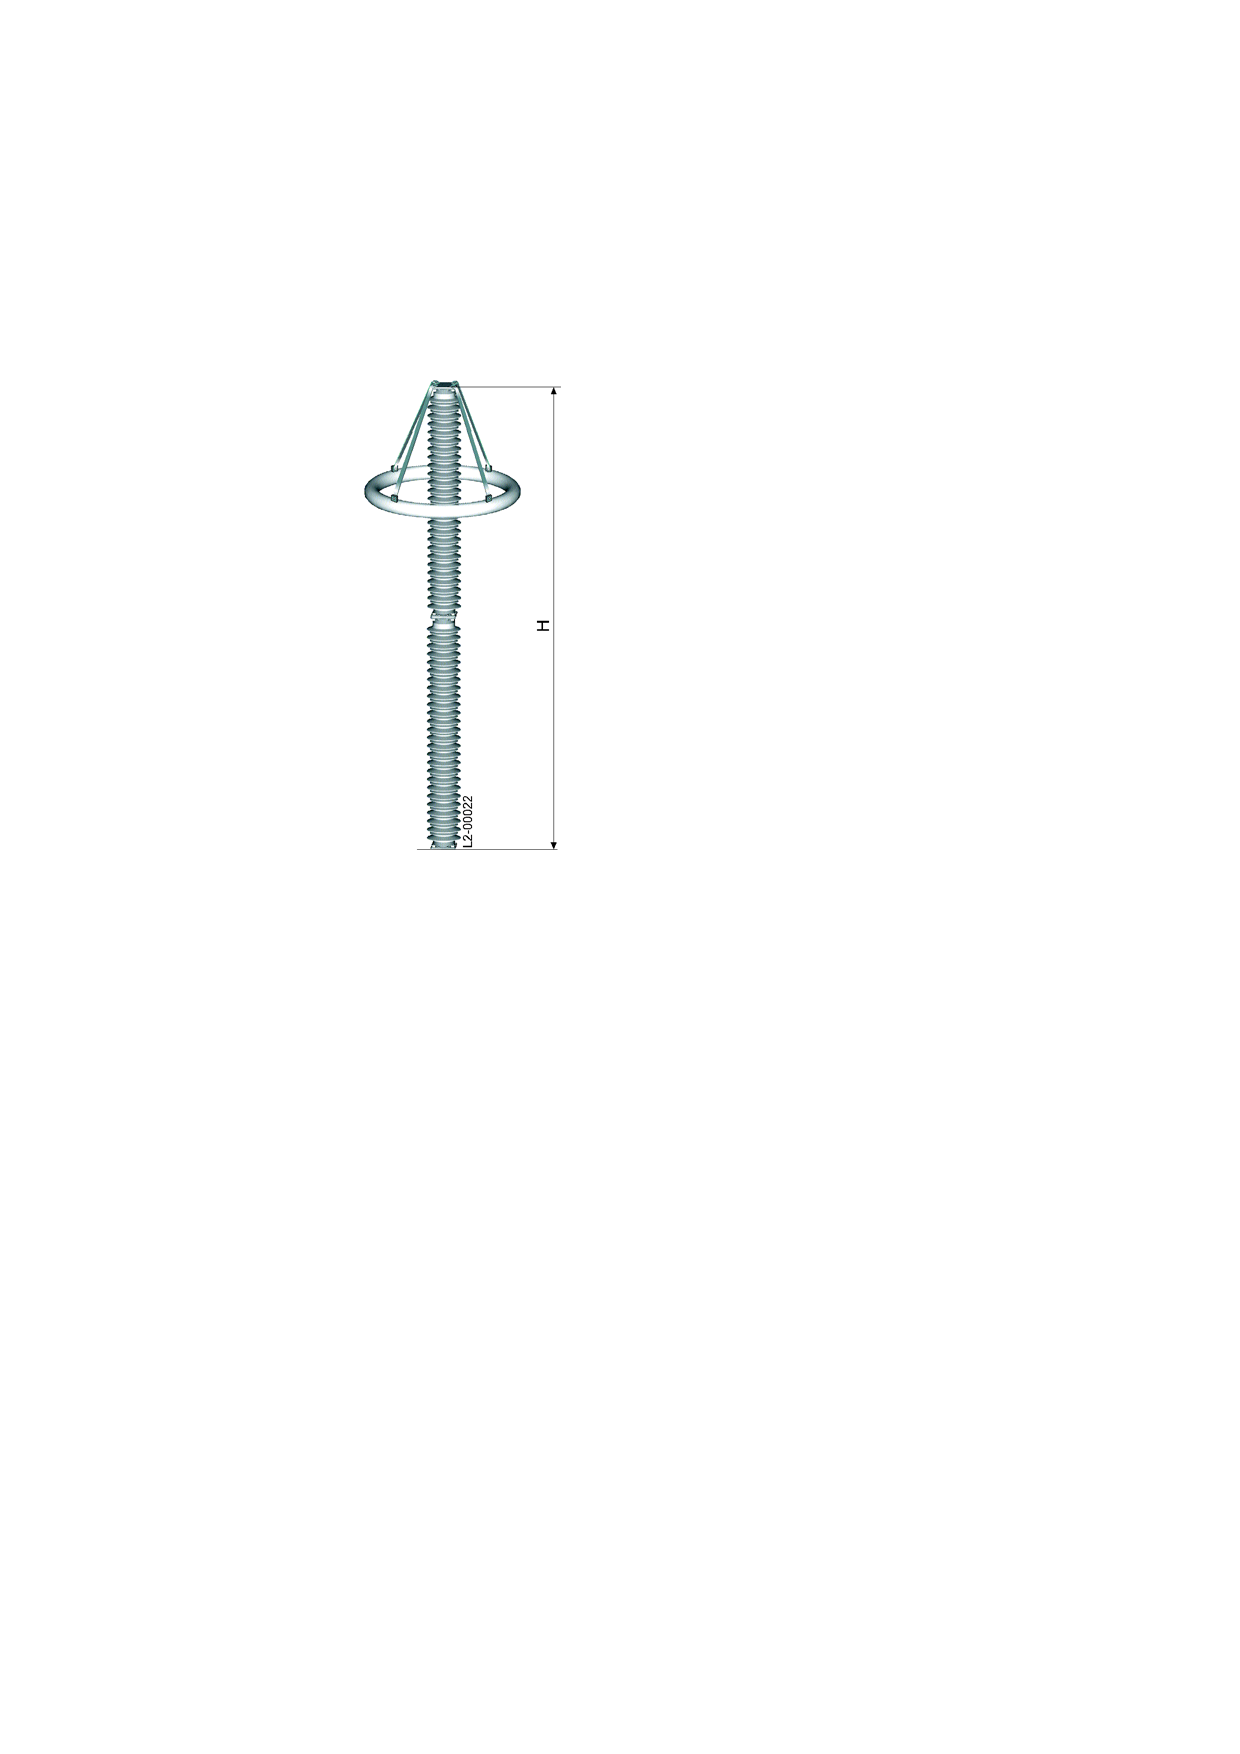
\includegraphics[width=2.7cm]{pararaio.pdf}
			\label{fig:pararaioA}
			}
			\subfloat[Placa de identificação] {
			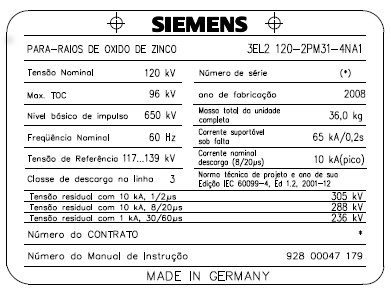
\includegraphics[width=8cm]{pararaio.jpg}
			\label{fig:pararaioB}
			}
			% \legend{Fonte: Do autor}
		\end{figure}

	\section{Muflas e Terminações}

	\section{Condutores}

	\section{Transformador de Corrente (TC)}
		Um transformador de corrente ou simplesmente TC é um dispositivo que reproduz no seu circuito secundário, a corrente que circula em um enrolamento primário com sua posição vetorial substancialmente mantida, em uma proporção definida, conhecida e adequada. Os transformadores de corrente, também chamados de transformadores de instrumentos, utilizados em aplicações de alta tensão (situações essas onde circulam, frequentemente, altas correntes), fornecem correntes suficientemente reduzidas e isoladas do circuito primário de forma a possibilitar o seu uso por equipamentos de medição, controle e proteção.

		\subsection{Características construtivas}
			A seguir apresenta-se as diferentes formas para diferentes usos do TC.

			\subsubsection{Formas Construtivas}
				\paragraph*{a)\indent TC tipo barra}
					É aquele cujo enrolamento é constituído por uma barra fixada através do núcleo do transformador, conforme mostrado na \autoref{fig:tca}.
					\begin{figure}[htb]
						\caption{TC tipo barra}
						\centering
						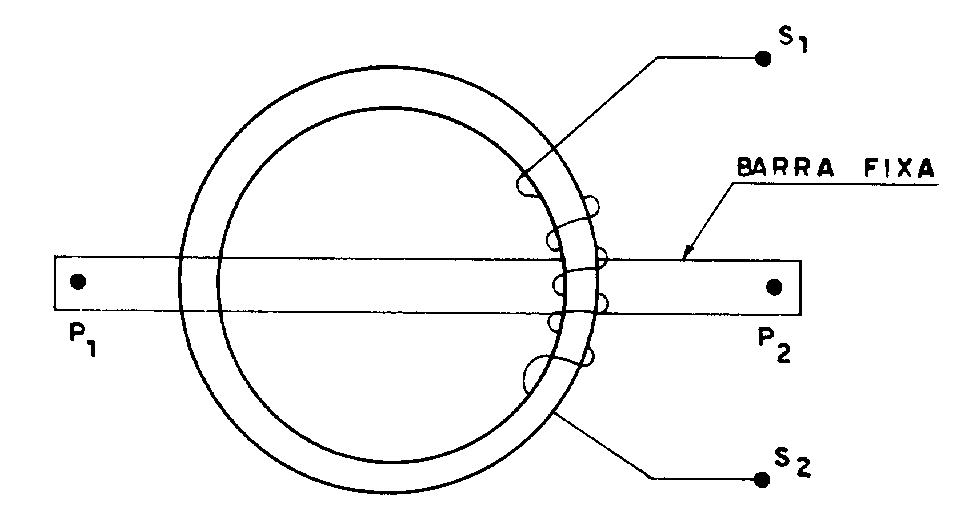
\includegraphics[width=5.4cm]{TC(1).png}
						% \legend{Fonte: Do autor}
						\label{fig:tca}
					\end{figure}
				\paragraph*{b)\indent TC tipo enrolado}
					É aquele cujo enrolamento é constituído de uma ou mais espiras envolvendo o núcleo do transformador, confomre ilustrado na \autoref{fig:tcb}.
					\begin{figure}[htb]
						\caption{TC tipo enrolado}
						\centering
						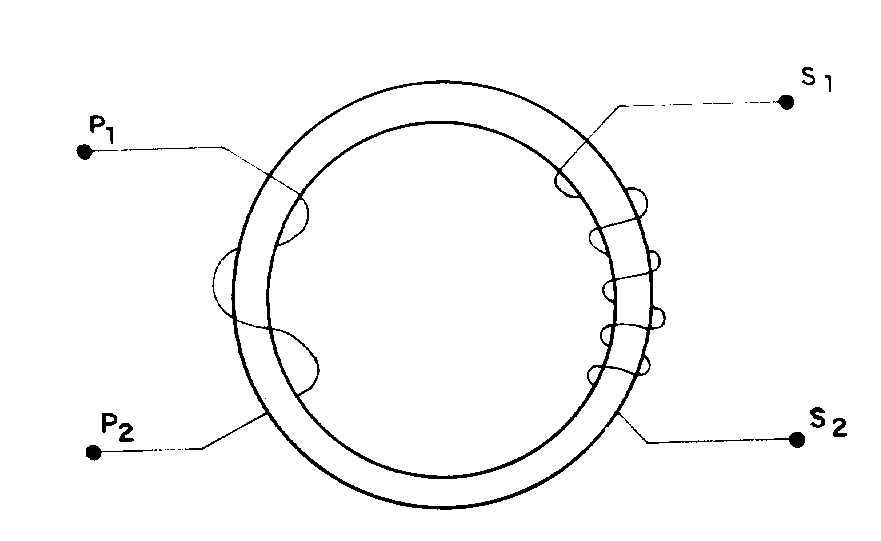
\includegraphics[width=5.4cm]{TC(2).png}
						% \legend{Fonte: Do autor}
						\label{fig:tcb}
					\end{figure}
				\paragraph*{c)\indent TC tipo janela}
					É aquele que não possui o primário fixo no transformador e é constituído de uma abertura através do núcleo, por onde passa o condutor que forma o circuito primário, conforme apresenta na \autoref{fig:tcc}.
					\begin{figure}[htb]
						\caption{TC tipo janela}
						\centering
						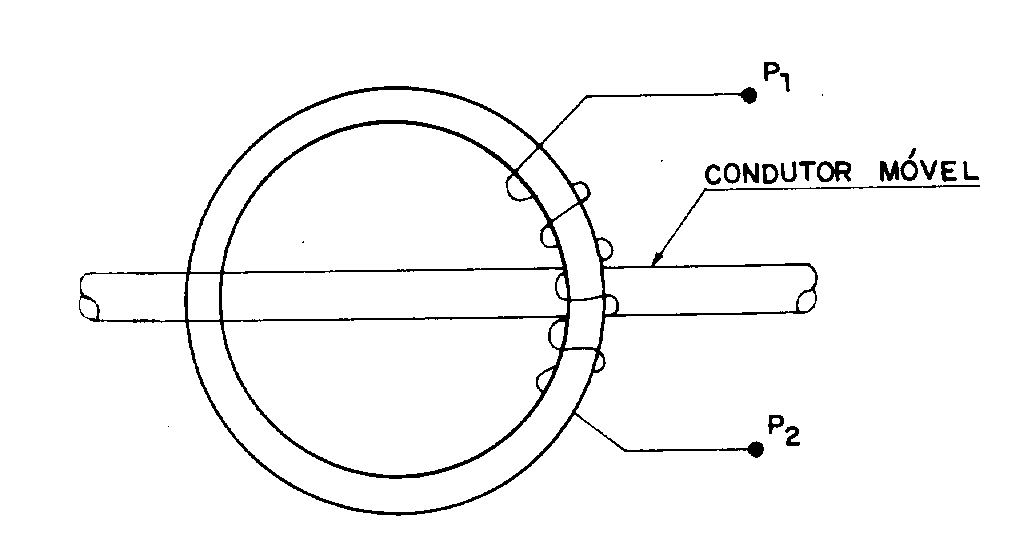
\includegraphics[width=5.4cm]{TC(3).png}
						% \legend{Fonte: Do autor}
						\label{fig:tcc}
					\end{figure}
				\paragraph*{d)\indent TC tipo bucha}
					É aquele cuja características são semelhantes às do tc do tipo barra, porém sua instalação é feita na bucha dos equipamentos, que funcionan como enrolamento primário, de acordo com a \autoref{fig:tcd}.
					\begin{figure}[htb]
						\caption{TC tipo bucha}
						\centering
						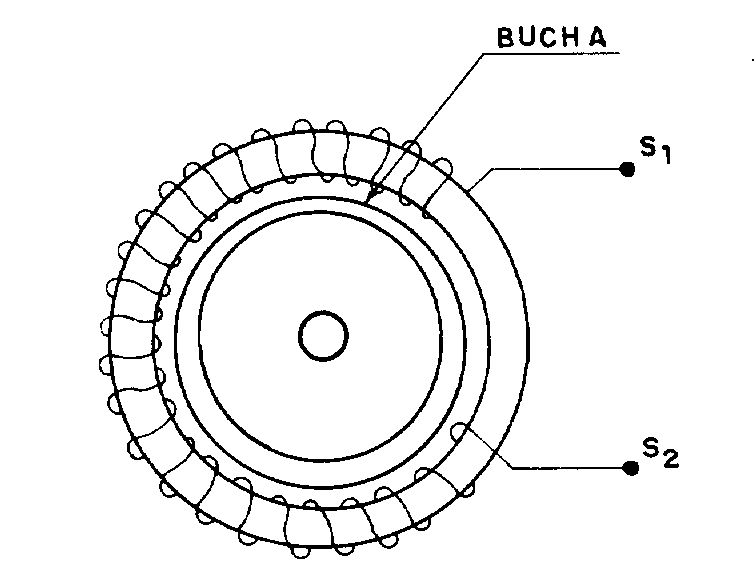
\includegraphics[width=5.4cm]{TC(4).png}
						% \legend{Fonte: Do autor}
						\label{fig:tcd}
					\end{figure}
				\paragraph*{e)\indent TC tipo núcleo dividido}
					É aquele cujas características são semelhantes às do tipo janela, em que o núcleo pode ser separado para permitir envolver o condutor que funciona como enrolamento primário, conforme se mostra na \autoref{fig:tce}.
					\begin{figure}[htb]
						\caption{TC tipo núcleo dividido}
						\centering
						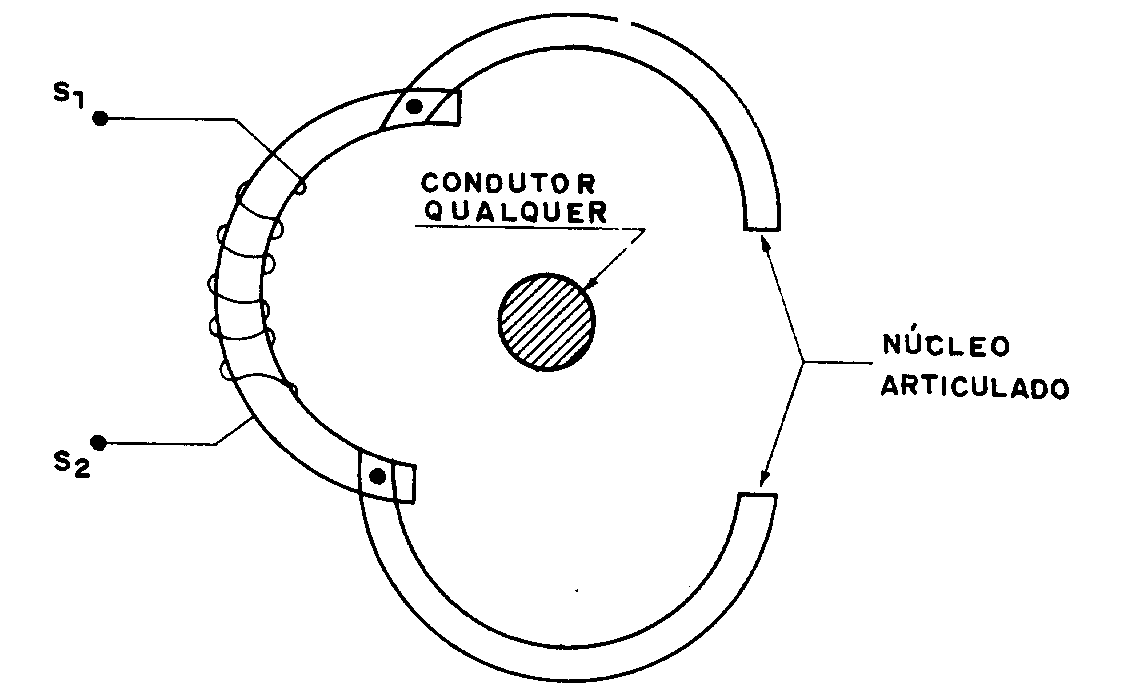
\includegraphics[width=5.4cm]{TC(5).png}
						% \legend{Fonte: Do autor}
						\label{fig:tce}
					\end{figure}
				\paragraph*{f)\indent TC tipo vários enrolamentos primários}
					É aquele constituído de vários enrolamentos primários montados isoladamente e apenas um enrolamento secundário, conforme a \autoref{fig:tcf}.
					\begin{figure}[htb]
						\caption{TC tipo vários enrolamentos primários}
						\centering
						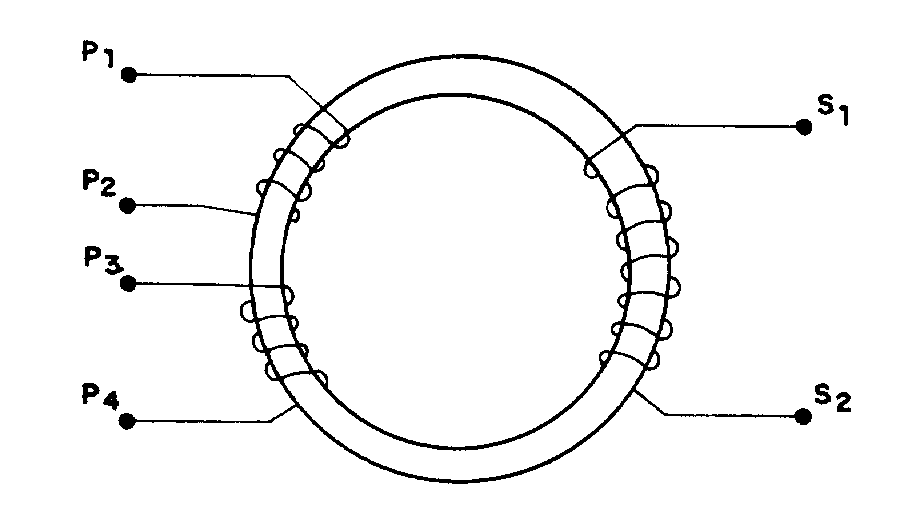
\includegraphics[width=5.4cm]{TC(6).png}
						% \legend{Fonte: Do autor}
						\label{fig:tcf}
					\end{figure}
				\paragraph*{g)\indent TC tipo vários núcleos secundários}
					É aquele constituído de dois o mais núcleos ssecundários montados isoladamente formando com o enrolamento primário, um só conjunto, conforme se mostra na \autoref{fig:tcg}.
					\begin{figure}[htb]
						\caption{TC tipo vários núcleos secundários}
						\centering
						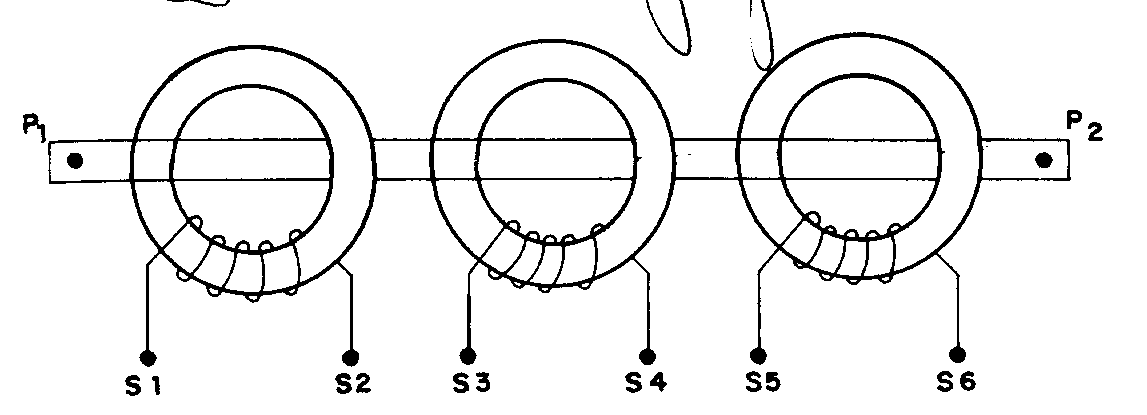
\includegraphics[width=5.4cm]{TC(7).png}
						% \legend{Fonte: Do autor}
						\label{fig:tcg}
					\end{figure}
				\paragraph*{h)\indent TC tipo vários enrolamentos secundários}
					É aquele constituído de um núcleo envolvido pelo enrolamento primário e vários enrolamentos secundários, conforme se mostra na \autoref{fig:tch}, e que podem ser ligados em série ou paralelo.
					\begin{figure}[htb]
						\caption{TC tipo vários enrolamentos secundários}
						\centering
						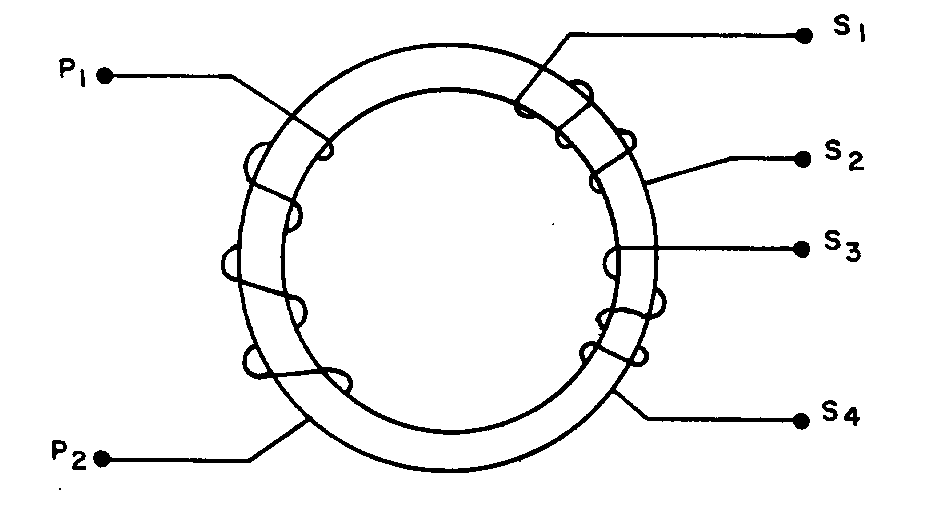
\includegraphics[width=5.4cm]{TC(8).png}
						% \legend{Fonte: Do autor}
						\label{fig:tch}
					\end{figure}
				\paragraph*{i)\indent TC tipo derivação no secundário}
					É aquele constituído de um único núcleo envolvido pelo enrolamentos primário e secundário, sendo este promovido de uma ou mais derivações. Entretanto, o primário pode ser constituído de um ou mais enrolamentos, conforme se mostra na \autoref{fig:tcf}. Como os ampères-espiras variam em cada relação de transformadores considerada, somente é garantida a classe de  exatidão do equipamento para a derivação que contiver o maior número de espiras. A versão desse tipo de TC é apresentado na \autoref{fig:tci}.  
					\begin{figure}[htb]
						\caption{TC tipo derivação no secundário}
						\centering
						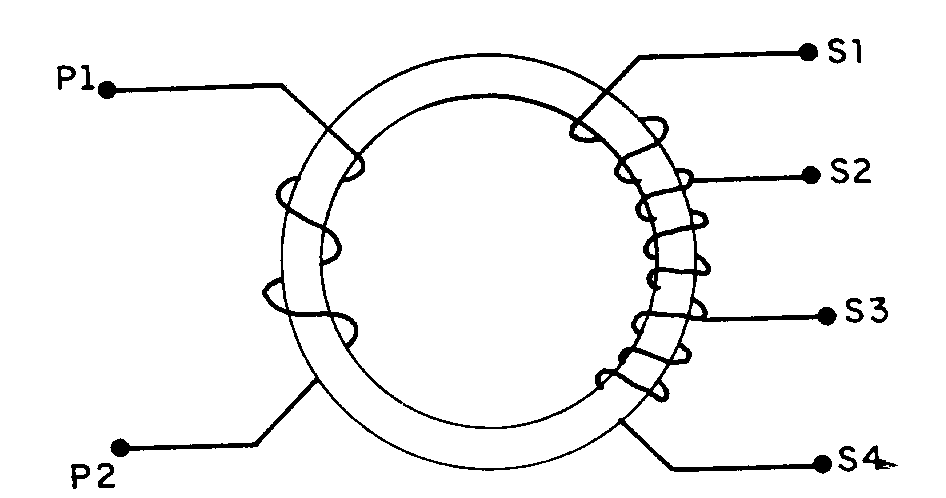
\includegraphics[width=5.4cm]{TC(9).png}
						% \legend{Fonte: Do autor}
						\label{fig:tci}
					\end{figure}
				\paragraph*{j)\indent TC de barra do tipo relação múltiplas com primário em várias seções}
					É aquele constituído de múltiplas barras no primário que podem ser ligadas em série-paralelo formando múltiplas relações.
			
			\subsubsection{Tipos de isolamento}
				\paragraph*{a)\indent TCs de baixa tensão}
					Os núcleo e os enrolamentos são encapsulados em resina epóxi que os torna rígidos, tornando-os compactos com características eletromecânicas de grande desempenho. Porém o epóxi tem a desvantagem de ser descartável depois de uma falha interna não sendo possível sua recuperação.
				\paragraph*{b)\indent TCs de média e alta tensão}
					Para a média tensão o isolamento pode ser em resinas sintéticas e a óleo mineral isolante, geralmente imerso num tanque metálico cheio de óleo. Agora os terminais constituídos por isoladores de porcelana.\par
					Para a alta tensão é usado porcelana-óleo e a hexafluoreto de enxofre ($SF_6$).\par

		\subsection{Características Elétricas}
			A simbologia padrão dos transformadores de corrente mostra os terminais primários de alta tensão H1 e H2 e os terminais secundários X1 e X2, como visto na \autoref{fig:tc1}.

			\begin{figure}[htb]
				\caption{Simbologia e circuito equivalente simplificado do TC}
				\centering
				\subfloat [Simbologia]{
				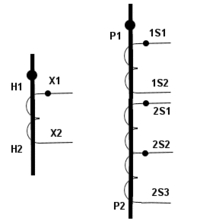
\includegraphics[width=5cm]{tca.jpg}
				\label{fig:tc1}
				}
				\subfloat [Circuito equivalente]{
				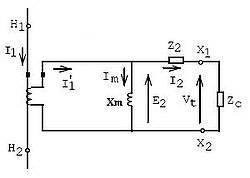
\includegraphics[width=5.8cm]{tcb.jpg}
				\label{fig:tc2}
				}
				% \legend{Fonte: Do autor}
			\end{figure}
			
			O ponto, para transformadores com polaridade aditiva, indica onde entra a corrente no primário e onde sai a corrente no secundário (defasagem de 180º). Modelos industriais de TC’s têm os terminais de alta tensão marcados como P1 e P2 (Primário 1 e Primário 2), sendo que em muitos casos pode haver diferentes ligações do circuito primário que permitam alterar a relação de transformação. Os terminais secundários são marcados como 1s1, 1s2, 2s2 (número, algarismo, número), indicando respectivamente o número do enrolamento, o símbolo de terminal secundário (s) e o número da derivação do terminal secundário.\par
			\begin{figure}[htb]
			  \caption{Placa de identificação de um TC utilizado no barramento de 138 kV}
			  \centering
			  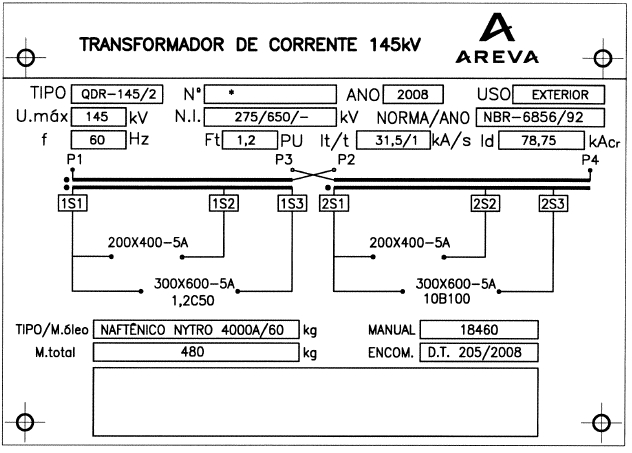
\includegraphics[width=10.8cm]{placatc.jpg}
			% \legend{Fonte: Do autor}
			  \label{fig:placatc}
			\end{figure}

			O circuito equivalente aproximado para um transformador de corrente é mostrado na Figura 10, onde a transformação da corrente entre os circuitos primário e secundário é feita sem perdas. A impedância de dispersão do primário Z1 é multiplicada pelo quadrado da relação $N^{2}$ quando referida ao secundário. A impedância de dispersão secundária é Z2. Os componentes de perdas no núcleo por correntes parasitas e por magnetização são dados por Zm e a impedância de carga é dada por Zc. Este circuito generalizado pode ser simplificado como mostrado no esquema ao lado. A impedância primária Z1 pode ser desprezada, uma vez que o reduzido número de espiras no primário (o que é verdadeiro para a maioria dos TC’s comerciais) tem pequena resistência e pouca dispersão. A corrente através do ramo magnetizante Xm é Im, chamada corrente de excitação. A corrente de excitação é atrasada de 90º em relação a V1'.\par
			\begin{figure}[htb]
			  \caption{Foto de um Transformador de Corrente}
			  \centering
			  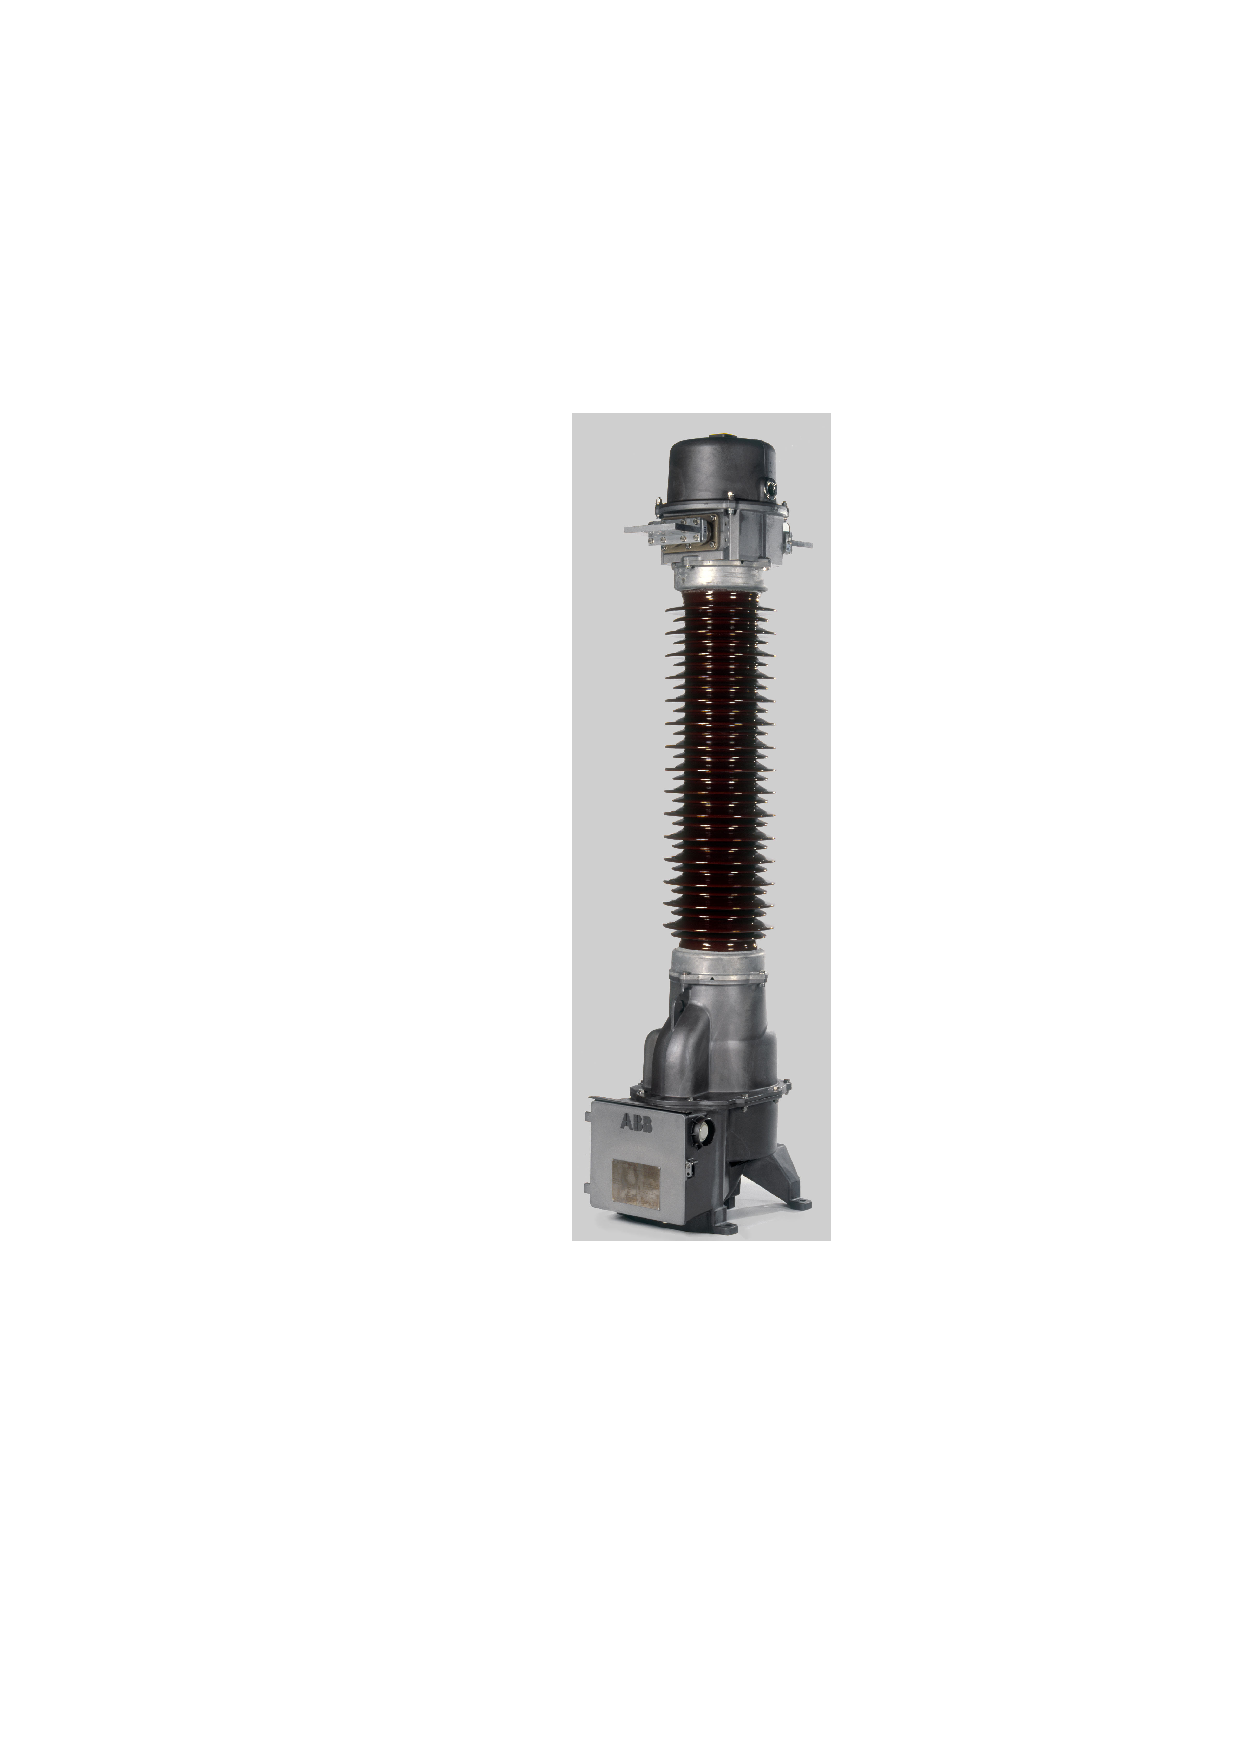
\includegraphics[width=3cm]{fototc.pdf}
			% \legend{Fonte: Do autor}
			  \label{fig:fototc}
			\end{figure}

		\subsection{Classificação}
			\subsubsection{TCs para serviço de medição}
				São os transforadores cuja função é medir, requer reproduzir fielmente a magnitude e o ângulo de fase da corrente, sua precisão deve ser garantida desde uma pequena fração de de corrente nominal da ordem de 10\% até o excesso de corrente da ordem de 20\%, sobre o valor nominal.\cite{apuntesmeza}\par
				\subsubsubsection{Fator de sobrecorrente}
				Além de representar uma elevada segurança aos operadores e leituristas, os TCs têm a finalidade de proteger os instrumentos de medida contra sobrecargas ou sobrecorrentes de valores muito elevados. Isto é possível, porque o seu núcleo é especificado para entrar em saturação para correntes superiores à corrente nominal vezes o fator de sobrecorrente, conforme se pode mostrar na \autoref{eq:fsobrecorrente}.
				\begin{equation} \label{eq:fsobrecorrente}
					F_{s} = \frac{I_{ps}}{I_{np}}
					\end{equation}

			\subsubsection{TCs para serviço de proteção}
				São os transformadores cuja função é proteger um circuito, requer conservar sua fidelidade até um valor de vinte vezes a magnitude de corrente nominal, quando trata-se de grande redes com altas correntes poder ser necessário requerer trinta vezes a corrente nominal.\par
				No caso dos relés de sobrecorrente, só importa a relação de transformação, mas em outros tipos de relés, como pode ser os de impedância, é requerido além da relação de transformação, manter o erro do ângulo de fase dentro dos valores predeterminados.\cite{apuntesmeza}\par

	\section{Transformador de Potencial (TP)}

	\section{Chave seccionadora}

	\section{Painéis}

	\section{Disjuntor}

	\section{Transformador de Potência}

	\section{Capacitores de Potência}

	\section{Resistores de Aterramento}

	\section{Reguladores de Tensão}

	\section{Religadores Automáticos}

	\section{Relés}


% ---------------------------------------------------
% Capítulo 2
% ---------------------------------------------------

\chapter{Projeto de subestações de alta tensão}
\label{chap:projSEAT}
	\begin{mdframed}[hidealllines=true,backgroundcolor=blue!20]
	\lipsum
	\end{mdframed}

% ---------------------------------------------------
% Capítulo 3
% ---------------------------------------------------

\chapter{Problemática da Demanda de Carga da Subestação Camboriú (CBU) -- SC}
\label{chap:demCarga}
	\begin{mdframed}[hidealllines=true,backgroundcolor=blue!20]
	\lipsum
	\end{mdframed}

% ---------------------------------------------------
% Capítulo 4
% ---------------------------------------------------

\chapter{Solução de Ampliação para a Subestação Camboriú}
\label{chap:solAmp}
	\begin{mdframed}[hidealllines=true,backgroundcolor=blue!20]
	\lipsum
	\end{mdframed}

% ---------------------------------------------------
% Capítulo 5
% ---------------------------------------------------

\chapter{Como é feito em outras partes do mundo}
\label{chap:asbuiltAbroad}
	\begin{mdframed}[hidealllines=true,backgroundcolor=blue!20]
	\lipsum
	\end{mdframed}


% ---------------------------------------------------
% Conclusão
% ---------------------------------------------------
\chapter*[Conclusão]{Conclusão}
\addcontentsline{toc}{chapter}{Conclusão}
	\begin{mdframed}[hidealllines=true,backgroundcolor=blue!20]
	\lipsum
	\end{mdframed}


\bibliography{refs}
\end{document}



%\begin{figure}[htb]
%	\caption{Sinal de ECG}
%	\centering
%	\includegraphics[width=16cm]{matlab1.pdf}
%	\legend{Fonte: Do autor}
%	\label{fig:matlab1}
%\end{figure}

